\documentclass{beamer}
\usepackage{media9}
\usepackage{animate}
\usetheme{Berkeley}
\title{Sampling from High Dimensional Distributions}
\subtitle{A Gradient Based Approach}
\author{Bill DeRose \\ Gabe Chandler}
\date{\today}

\begin{document}

\frame{\titlepage}

\section[Outline]{}
\frame{\tableofcontents}

\section{Introduction}
\subsection{Randomness}
\frame
{
  \frametitle{What is random?}
  \begin{figure}[!htbp]
   	\centering
   		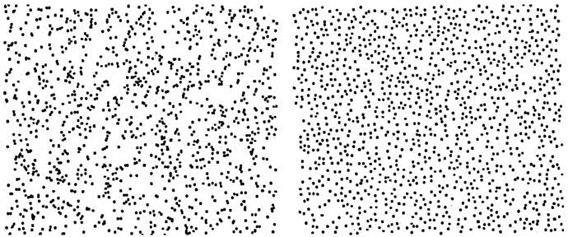
\includegraphics[scale=0.6]{images/random?} 
  	 \label{fig:example}
   \end{figure}
}
\section{Sampling Methods}
\subsection{Inverse Transform}
\frame
{
  \frametitle{Drawing Samples from a Distribution}
	\begin{itemize}
		\item Assume we have $U \sim \mbox{Unif}[0, 1]$.
		\begin{itemize}
			\item Where does this get us?
		\end{itemize}
		\pause
		\item Cumulative distribution function: $z = h(x) = \int_{-\infty}^x p(\hat{x}) \,d\hat{x}$
		\pause		
		\item Idea: transform the uniform random variables using the inverse of the 
		indefinite integral of the desired distribution. 
		$$x = h^{-1}(z) = h^{-1}\bigg( \int_{-\infty}^x p(\hat{x}) \,d\hat{x}\bigg)$$
	\end{itemize}
}
\frame{
	\frametitle{Inverse Transform Example}
   	\centering
   	\includegraphics<1>[scale=0.25]{images/normal_pdf.jpeg} 
	\includegraphics<2>[scale=0.25]{images/normal_pdf_and_cdf.jpeg} 
	\includegraphics<3>[scale=0.25]{images/inverse}
	\includegraphics<4>[scale=0.25]{images/inverse_mapping}
}
\frame{
	\frametitle{Inverse Transform Example}
   	\centering
	\animategraphics[autoplay, loop, width=.5\linewidth]{25}{animations/inverse_transform/Rplot}{1}{1000}
}
\subsection{MCMC}
\frame{
	\frametitle{Look Ahead}
	\begin{itemize}[<+->]
	\item Inverse transform requires us to evaluate an indefinite integral -- sometimes infeasible. 
	\item My thesis: deep dive into sampling methods for complex distributions and high dimensional space
		\begin{itemize}
			\item Gibbs Sampling
			\item Slice Sampling
			\item Markov Chain Monte Carlo
			\item Hamiltonian Monte Carlo
		\end{itemize}
	\end{itemize}
}
\end{document}
